\chapter{Implementacja}

\section{Konfiguracja środowiska}
Do stworzenia bota użyto języka Python w wersji 3. W tym celu zainstalowano najnowszą wersję, którą można znaleźć na oficjalnej stronie: \texttt{https://www.python.org/}.
Aby ułatwić pracę w środowisku, dodatkowo zainstalowano managera paczek do Python’a - PIP. Instrukcje dotyczące manualnej instalacji można znaleźć na oficjalnej stronie: \texttt{https://pypi.org/project/pip/}.

\section{Konfiguracja biblioteki ChatterBot}
Instalacja biblioteki ChatterBot jest bardzo prosta przy użyciu PIP. Całą bibliotekę można zainstalować jedną komendą:
\begin{center}
pip install chatterbot
\end{center}
Zainstalowaną bibliotekę można sprawdzić przy pomocy komendy:
\begin{center}
python -m chatterbot --version
\end{center}
Terminal powinien zwrócić aktualną wersję.

\section{Implementacja chatbota}

Pierwszym elementem programu było stworzenie obiektu chatbota. Wykonano to przy pomocy obiektu ChatBot z biblioteki ChatterBot. Podczas tworzenia obiektu chatbota można zainicjalizować go kilkoma parametrami.

\begin{figure}[ht]
	{\centering
		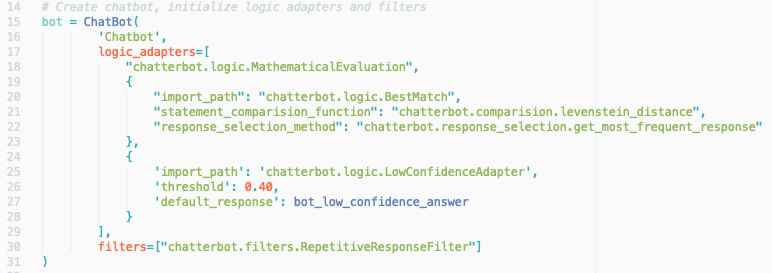
\includegraphics[width=0.9\linewidth]{rys/rys02/1}
	\caption{Tworzenie obiektu bota - kod źródłowy.}
	}
	\label{fig:bot1}
\end{figure}

\newpage

Pierwszym parametrem jest nazwa chatbota.
Kolejnym jest lista adapterów logicznych, których można podać inicjując bota. Nie są one obowiązkowe, ale bez ich określenia, stworzony bot będzie posiadał adaptery domyślne. Aby mieć większą kontrolę nad chatbotem, podano kilka adapterów:
\begin{itemize}
	\item MathematicalEvaluation - dzięki temu adapterowi bot jest w stanie odpowiadać na pytania rozwiązując proste operacje matematyczne. Np. na pytanie $2+2$, powinien zwrócić odpowiedź $4$, która jest prawidłowym wynikiem dodawania.

	\item BestMatch - adapter logiczny, który przy wybieraniu odpowiedzi wybiera tą która najlepiej pasuje do pytania lub po prostu jest tej odpowiedzi najbardziej pewny. Porównywanie odpowiedzi odbywa się przy użyciu algorytmu dogległości Levenstein'a (linia 20 kodu), a z pośród znalezionych odpowiedzi bot wybiera tą, która wystąpiła najczęsciej (linia 21 kodu).

	\item LowConfidenceAdapter - adapter odpowiadający za działanie w przypadku gdy bot nie jest pewny odpowiedzi na zadane pytanie. Adapter ten pozwala ustawić próg poniżej, którego bot nie jest w stanie odpowiedzieć i zwróci tekst informujący o tym np. \textit{Przepraszam ale nie jestem w stanie odpowiedzieć na to pytanie}.
\end{itemize}
Ostatnim parametrem są filtry. Tutaj dodano filtr RepetitiveResponseFilter, który zapobiega powtarzaniu tych samych odpowiedzi przez bota.

\subsection{Uczenie}
Kolejnym etapem jest uczenie bota. Uczenia można dokonać przy pomocy plików tekstowych, zawierających pytania i odpowiedzi w odbpowiednim schemacie. W tym celu stworzono folder, w którym umieszczono wszystkie pliki uczące w formacie \textit{txt}. 

\begin{figure}[ht]
	{\centering
		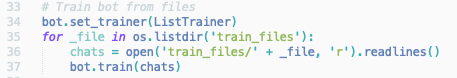
\includegraphics[width=0.7\linewidth]{rys/rys02/2}
	\caption{Uczenie bota - kod źródłowy.}
	}
	\label{fig:bot2}
\end{figure}

Program wczytuje wszystkie pliki w zadanym folderze, otwiera je w trybie odczytu i czyta wszystkie linie. Bot uczy się z każdego pliku, zapamiętuje pytania i odpowiedzi dodając je do bazy danych.

\subsection{Baza wiedzy}
W celu nauczenia bota odpowiedzi na pytania z różnych tematów przygotowano odpowiednie pliki w formacie tekstowym \textit{txt}. Każdy plik odpowiada za inny temat dialogu. Przygotowano odpowiednio dane o tematyce:
\\
\begin{center}
	\begin{tabular}{ll c c}
	- dostawa & 
	- konto klienta \\ [0.3cm]
	
	- płatności & 
	- powitania \\ [0.3cm]
	
	- pożegnania & 
	- promocje \\ [0.3cm]
	
	- reklamy & 
	- zwroty \\ [0.3cm]
	\end{tabular}
\end{center}


Format pliku to pytanie i odpowiedź w kolejnych liniach pliku. 

\begin{figure}[ht]
	{\centering
		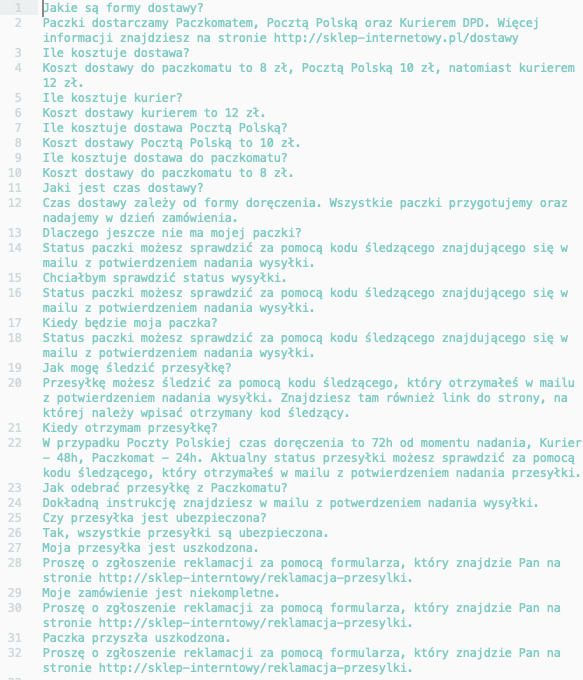
\includegraphics[width=0.9\linewidth]{rys/rys02/3}
	\caption{Przykładowy plik z danymi - dostawa.txt.}
	}
	\label{fig:bot3}
\end{figure}

\newpage


\subsection{Dialog bota z użytkownikiem}

\begin{figure}[ht]
	{\centering
		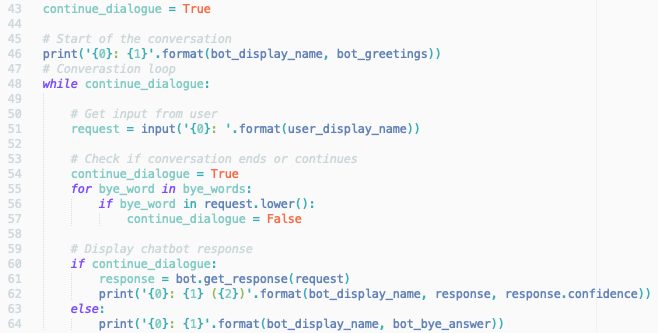
\includegraphics[width=0.9\linewidth]{rys/rys02/4}
	\caption{Dialog bota z użytkownikiem - kod źródłowy.}
	}
	\label{fig:bot4}
\end{figure}

Na samym początku bot zaczyna dialog witając użytkownika i czekając na wprowadzenie tekstu. Dialog zapętlony jest aż do momentu kiedy użytkownik zakończy konwersacje jednym z definiowanych słów pożegnalnych (do widzenia, żegnam, koniec). Po wprowadzeniu tekstu przez użytkownika sprawdzane jest czy nie zakończył on konwersacji. Jeżeli tak, bot żegna się i program kończy działania. W przeciwnym wypadku bot analizuje wprowadzony przez użytkownika tekst i wybiera najlepszą odpowiedź. Gdy pewność odpowiedzi bota jest większa niż przyjęty próg $0.4$, odpowiedź zostaje wyświetlona. Dla ułatwienia testowania, z każdą odpowiedzią bota na końcu wyświetlana jest jego pewność jako wartość z przedziału ${\{0,1\}}$.

\begin{figure}[ht]
	{\centering
		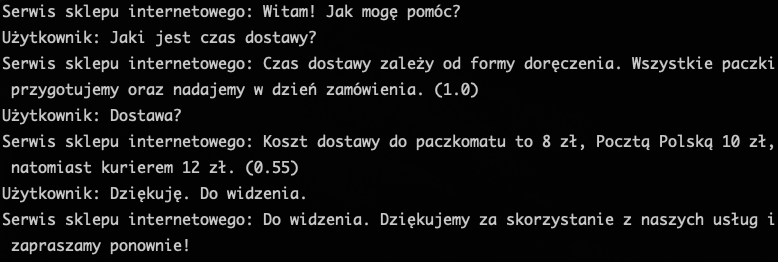
\includegraphics[width=0.9\linewidth]{rys/rys02/5}
	\caption{Przykładowy dialog.}
	}
	\label{fig:bot5}
\end{figure}
